\documentclass[12pt, fullpage,letterpaper]{article}
\usepackage[margin=1in]{geometry}
\usepackage{graphicx}
\title{CS6630 Visualization Fall 2017 Project Proposal\\ A Mirror of History}
\author{Yanqing Peng, Yuwei Wang}
\begin{document}
\maketitle

The title \textbf{A mirror of history} comes from the epitaph of Wei Zhen,
a famous Chinese historian:

\emph{``Using copper as a mirror allows one to keep his clothes neat. Using
history as a mirror allows one to see the future trends. Using a person as a
mirror allows one to see what is right and what is wrong.''}

\section{Basic Information}
\paragraph{Title} A Mirror of History
\paragraph{Group members}
\begin{itemize}
    \item Yanqing Peng, u1076076, yq.peng@utah.edu
    \item Yuwei Wang, u1140944, yuwei.utah@gmail.com
\end{itemize}
\paragraph{Github link} https://github.com/uvril/VisProject

\section{Background and Motivation}

History is always fascinating.  It's important to learn lessons from the past,
by understanding the causality behind historical events.  To learn about
history is to learn about humanity, which basically means developing an
understanding of ourselves.  Therefore, knowledge of history helps us prepare
better for future.

However, it can be boring to learn history by texts and numbers. We can know
from textbook that the British Empire used to rule 35,500,000 km$^2$ area of
land. But how large is it?  Showing a map of British Empire is much more
interesting than just telling the number.  Similarly, we know that the economy
of both Japan and Singapore grow dramatically after World War II, but both slow
down in 1990s.  How can we present a comparison between the economy development
of Japan and Singapore?  Showing the GDP table will be boring and hard to
understand.  Instead, showing a line chart for the GDP of Japan and Singapore
is much more clearer. Therefore, visualization is essential for learning history.

Our textbooks already contain plenty of figures to visualize history. However,
it's not enough. While learning history, people have different focuses.  Alice
is interested in the border of British Empire in 1913, while Bob wants to see a
map of French colonies in 1908. Charlie would like to know the comparison
between Japan and Singapore, while Eve is curious about the comparison between
India and Pakistan.  Only with interactive visualizations can one develops the
knowledge of history with his own interests.

The course project of CS6630 gives us a golden opportunity to learn better
about history.  We are willing to make a deeper insight into history, by
constructing an interactive visualization on history. We believe that the tools
we've learned from this course will help us fulfill our objectives.


\section{Project Objectives}
The main objective of this project is to interactively visualize the historical rise
and fall.  We would like to answer the following questions:
\begin{itemize}
    \item Show the historical world map at a specified year.

        Example: ``What is the world look like in 1939?.''

    \item For some desired attribute, visualize it on different countries in a specified year.

        Example: ``Show the population of all contries in 1945.''

    \item For a specified country, visualize a desired attribute over a specified time range.

        Example: ``Show the GDP of India from 1945 to 2017.''

    \item For a specified attribute, some specified countries and a specified time range, visualize the aggregated data.

        Example: ``Show the GDP of Brazil, India, China, Russia and South Africa from 1945 to 2017.''

    \item (Optional) Similar to the above question, but select the country by condition instead of directly specify the set of countries.

        Example: ``Show the Top 10 countries by GDP from 1945 to 2017.''

    \item (Optional) Show the impact of historical events.

        Example: ``For the event \emph{World War II}, highlight the envolved countries and the corresponding year range.
\end{itemize}

\section{Data}
Historical data are easy to retrieve, since they are actually public data that available to all.
Useful resources include:

\begin{itemize}
    \item Wikipedia, for statistical data (e.g. population).
    \item Thenmap.net, generates historical maps with GeoJSON/TopoJSON format.
    \item Educational resources and other resources (e.g. Chronas.org). There are plenty of educational resourses that can help us.
    \item Strategy games about history, (e.g. Crusader King, Europa Universalis, Heart of Irons, Victoria). Although the data from strategy games are not accurate, they can be use
        as a reference.
\end{itemize}

\section{Data Processing}
Since there are so many candidate data sources, we are unable to make it clear how to process data for now.
Basically, we wish to get the following datasets after data processing:
\begin{itemize}
    \item GeoJSON/TopoJSON files for country borders at different times.
    \item A CSV data for each contry to record its statistics (GDP/population/total area etc.) at different times.
    \item A data set that contains major historical events and their impacts.
\end{itemize}

We plan to use Python to pre-process the data into desired format before feeding it to Javascript.

\section{Visualization Design}

The visualization should contain the following parts:

\begin{itemize}
    \item A year chart that we can select a desired year from it.
        Basically it should be a row of years, and we can click on a desired year to select it.
        It should support zooming and sliding to help select a specific year.
    \item A map chart which covers the most area of the webpage.
        It shows the world map at the selected year.
        A country can be selected with a mouse click.
        We plan to add zooming functionality to make it easier to click on small countries.
    \item An information panel that displays the detailed information of the selected country at the selected year.
    \item An aggregation view chart that show some desired aggregation data based on the selection on countries and years.
    \item (Optional) A list that shows major historical events (e.g. wars). We can choose an interested event to see the details.
\end{itemize}

If we simply want to show the information for one country in one year, the
first three parts are already sufficient. The aggregation view chart answer
complicated questions such
as ``show a comparison between the economic of N. Korea and S. Korea from 1946
to 2012''.  Basically, these questions contain a set of countries, a set of
years, and a specified attribute.  We need to aggregate data based on the
selections and show an appropriate visualization of the aggregated data in the
aggregation view chart.

We designed three alternatives for our visualization.  The designs are show in
Figures \ref{fig:alt1}, \ref{fig:alt2} and \ref{fig:alt3} respectively in the
last pages of this report.  Please kindly refer to them.

\paragraph{Final Decision}

Based on the three alternatives, we present the final decision of visualization
design in Figure \ref{fig:final}. The final design incorporates the best
of the three alternatives.

\section{Must-Have Features}
A user should be able to:
\begin{itemize}
    \item Zoom and slide the year chart.
    \item Choose a desired year in the year chart. 
    \item See the world map of the selected year in the map chart.
    \item Select a country in the map chart.
    \item See the detailed information about the selected country in the information panel.
    \item Select several contries and select several years.
    \item Select a desired statistics (e.g. population), show the aggregated data based on the selections in the aggregation view chart.
\end{itemize}

\section{Optional Features}
A user may also be able to:
\begin{itemize}
    \item Zoom the map in order to see small countries.
    \item Select all countries that satifies a specified condition.
    \item Select from a list of major historical events. The impact of the selected event is somehow shown on the map chart and the information panel.
    \item Select other views of the map, e.g., a heat map of population. In this case an additional layer of heat map is shown above the map.
\end{itemize}

\section{Project Schedule}
\paragraph{Oct 30-Nov 5} Start data collection and data processing.
\paragraph{Nov 6-Nov 12} Finish data processing and webpage construction. A simple demo should be made before milestone.
\paragraph{Nov 13-Nov 19} Complete most must-have features.
\paragraph{Nov 20-Nov 26} Complete must-have features. If time permits, complete optional features.
\paragraph{Nov 27-Dec 1} Finalize the project.

\section{Figures}
\begin{figure}[h!]
    \begin{center}
        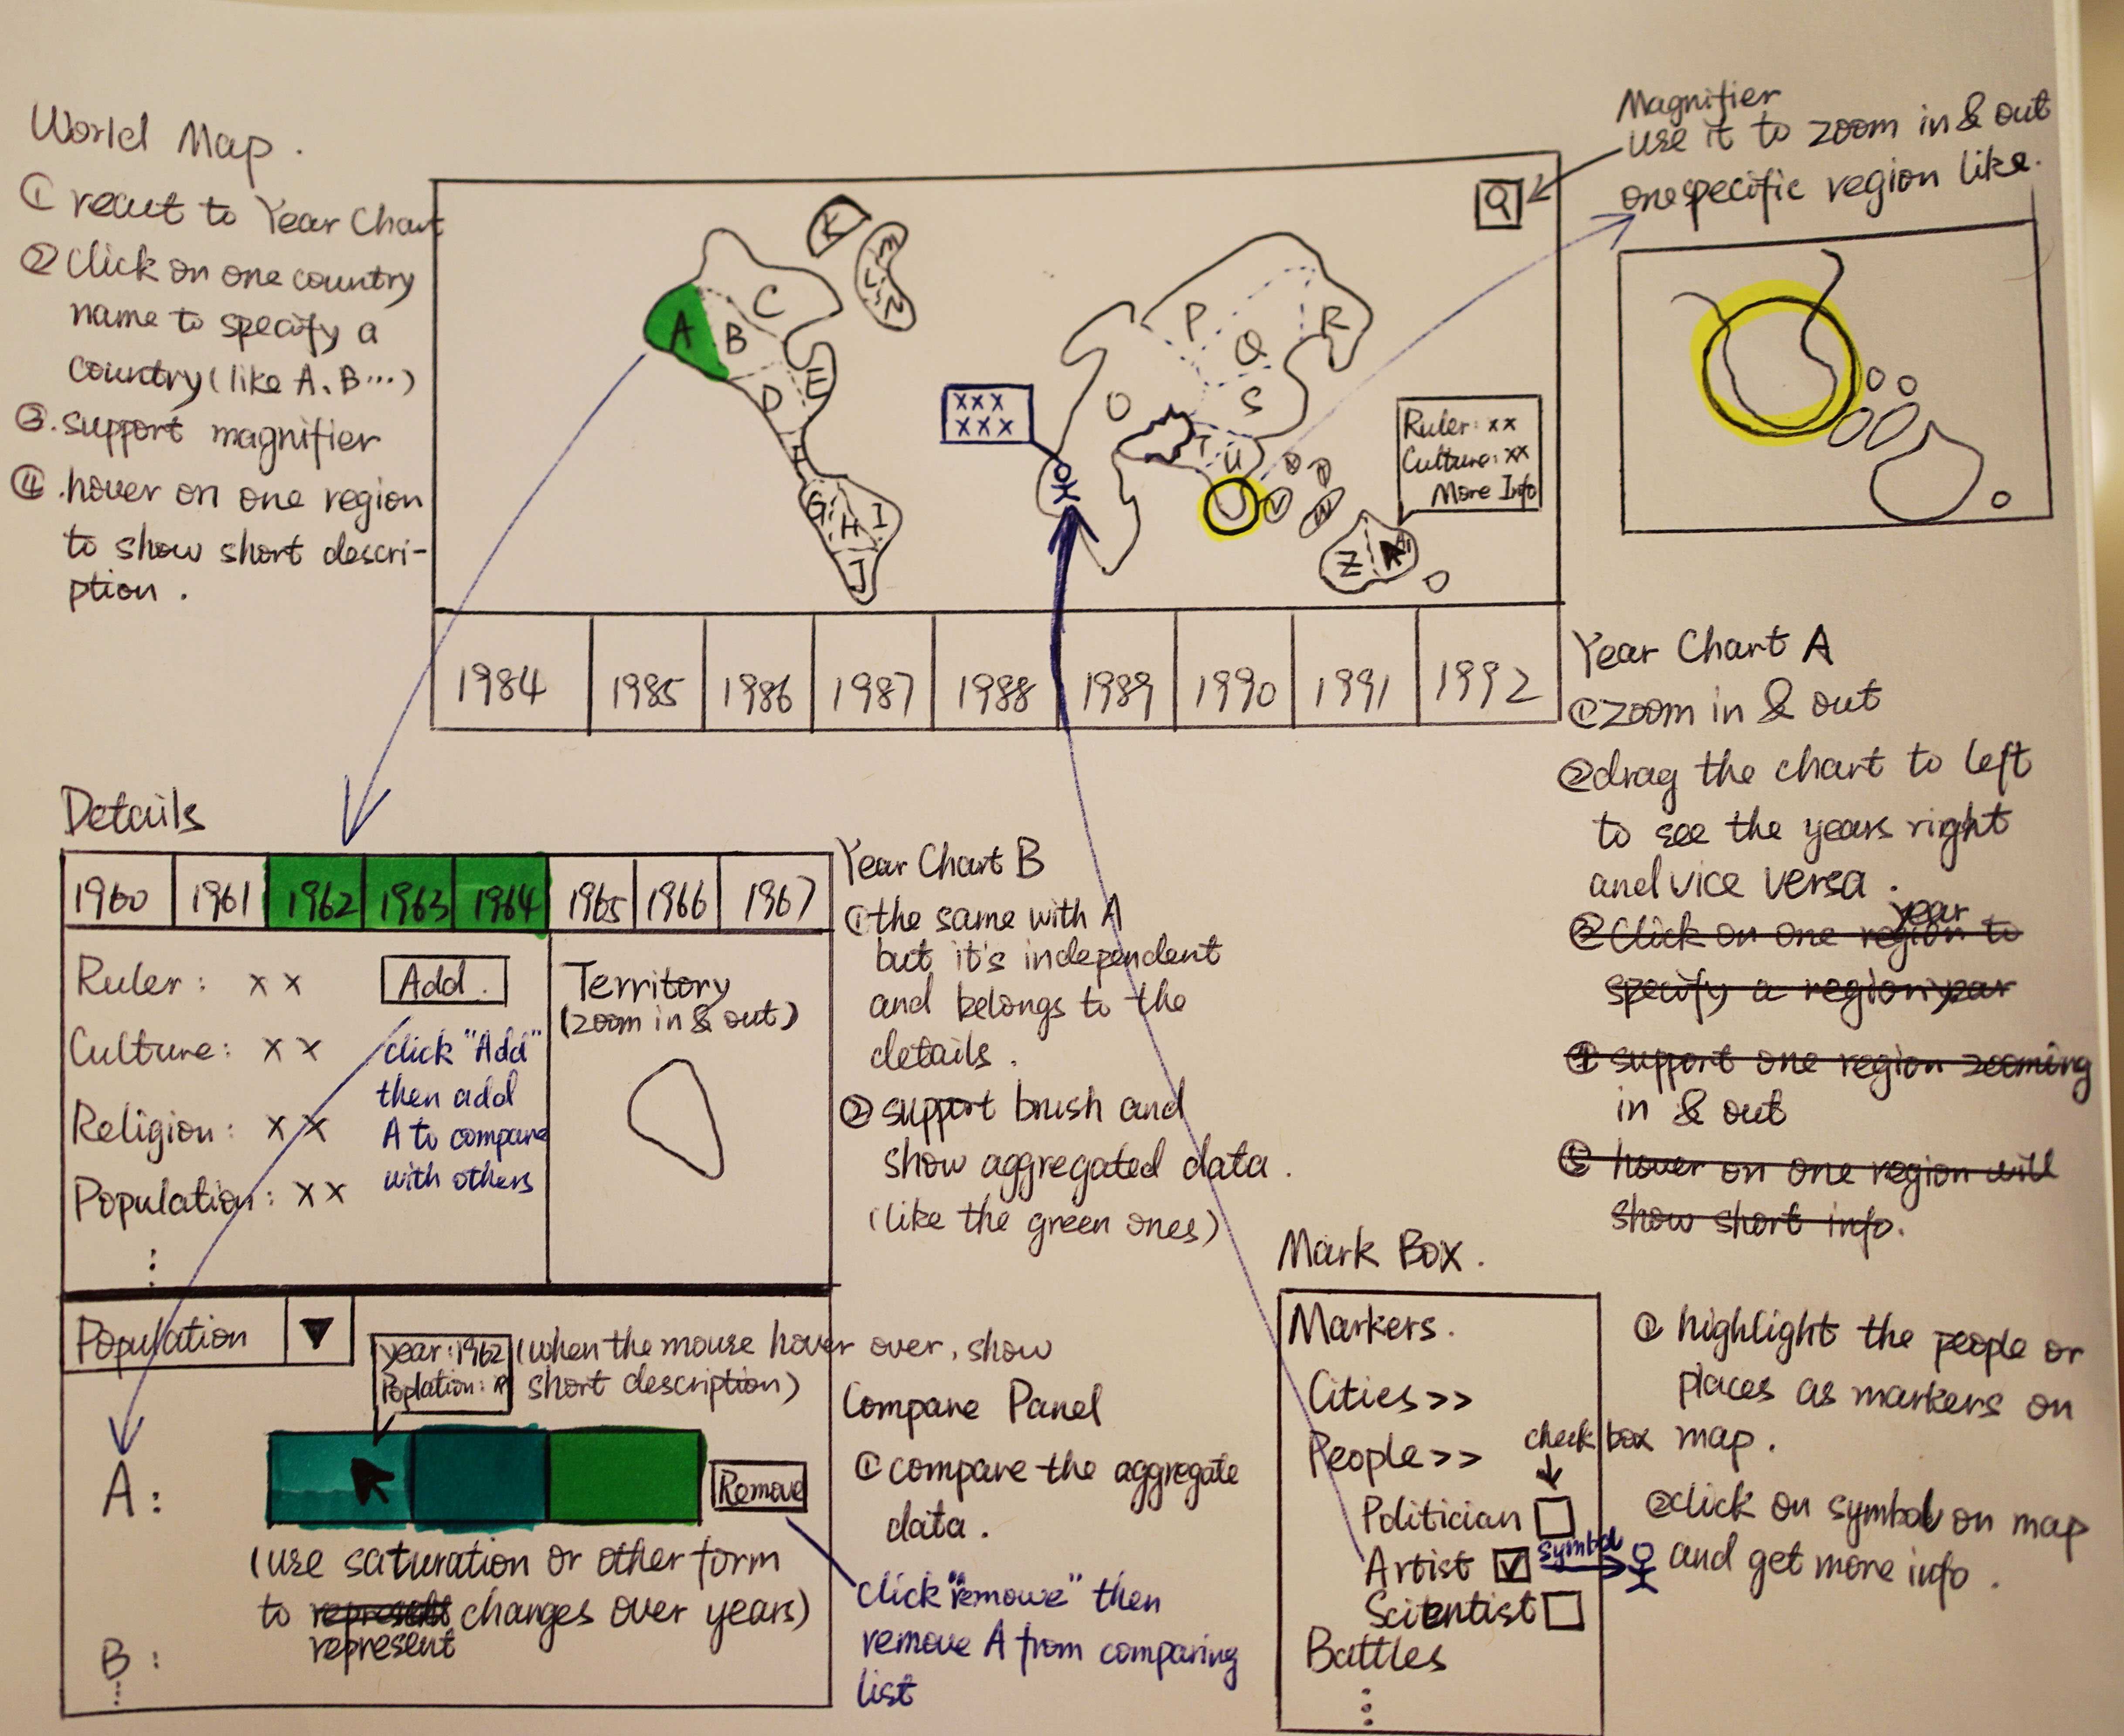
\includegraphics[width=\textwidth]{alternative1.JPG}
        \caption{Alternative 1}
        \label{fig:alt1}
    \end{center}
\end{figure}

\begin{figure}[h!]
    \begin{center}
        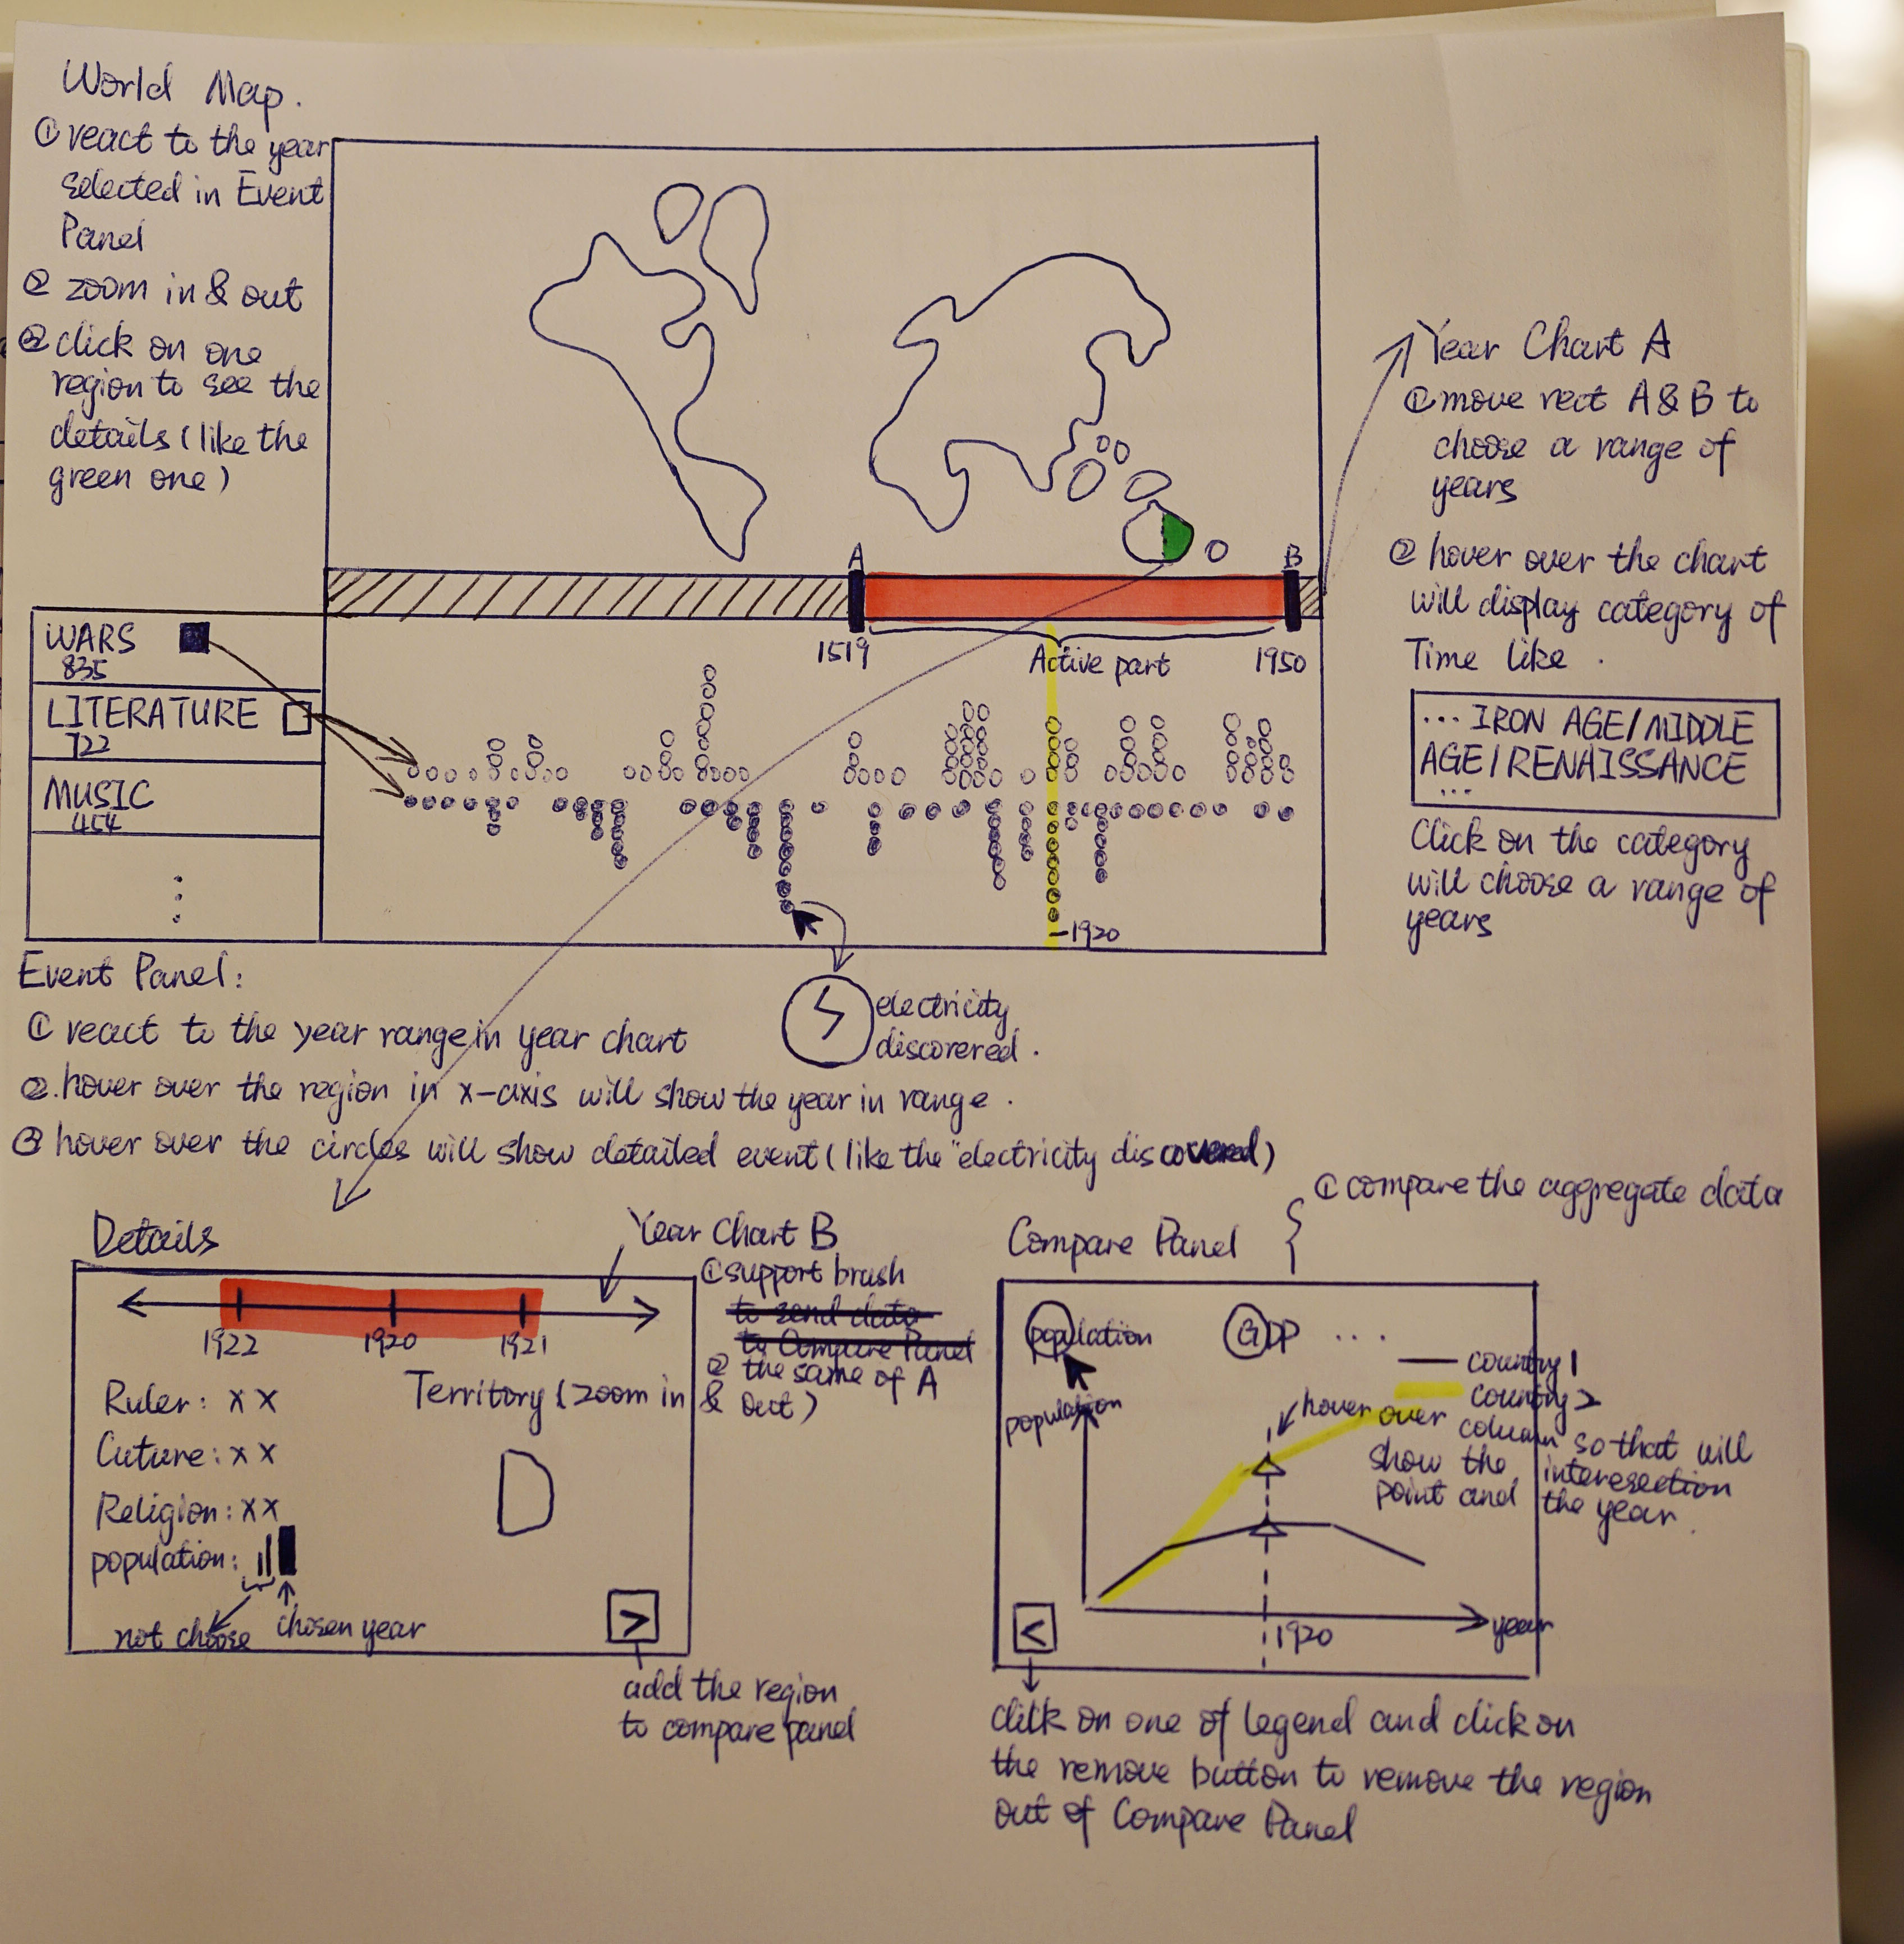
\includegraphics[width=\textwidth]{alternative2.JPG}
        \caption{Alternative 2}
        \label{fig:alt2}
    \end{center}
\end{figure}

\begin{figure}[h!]
    \begin{center}
        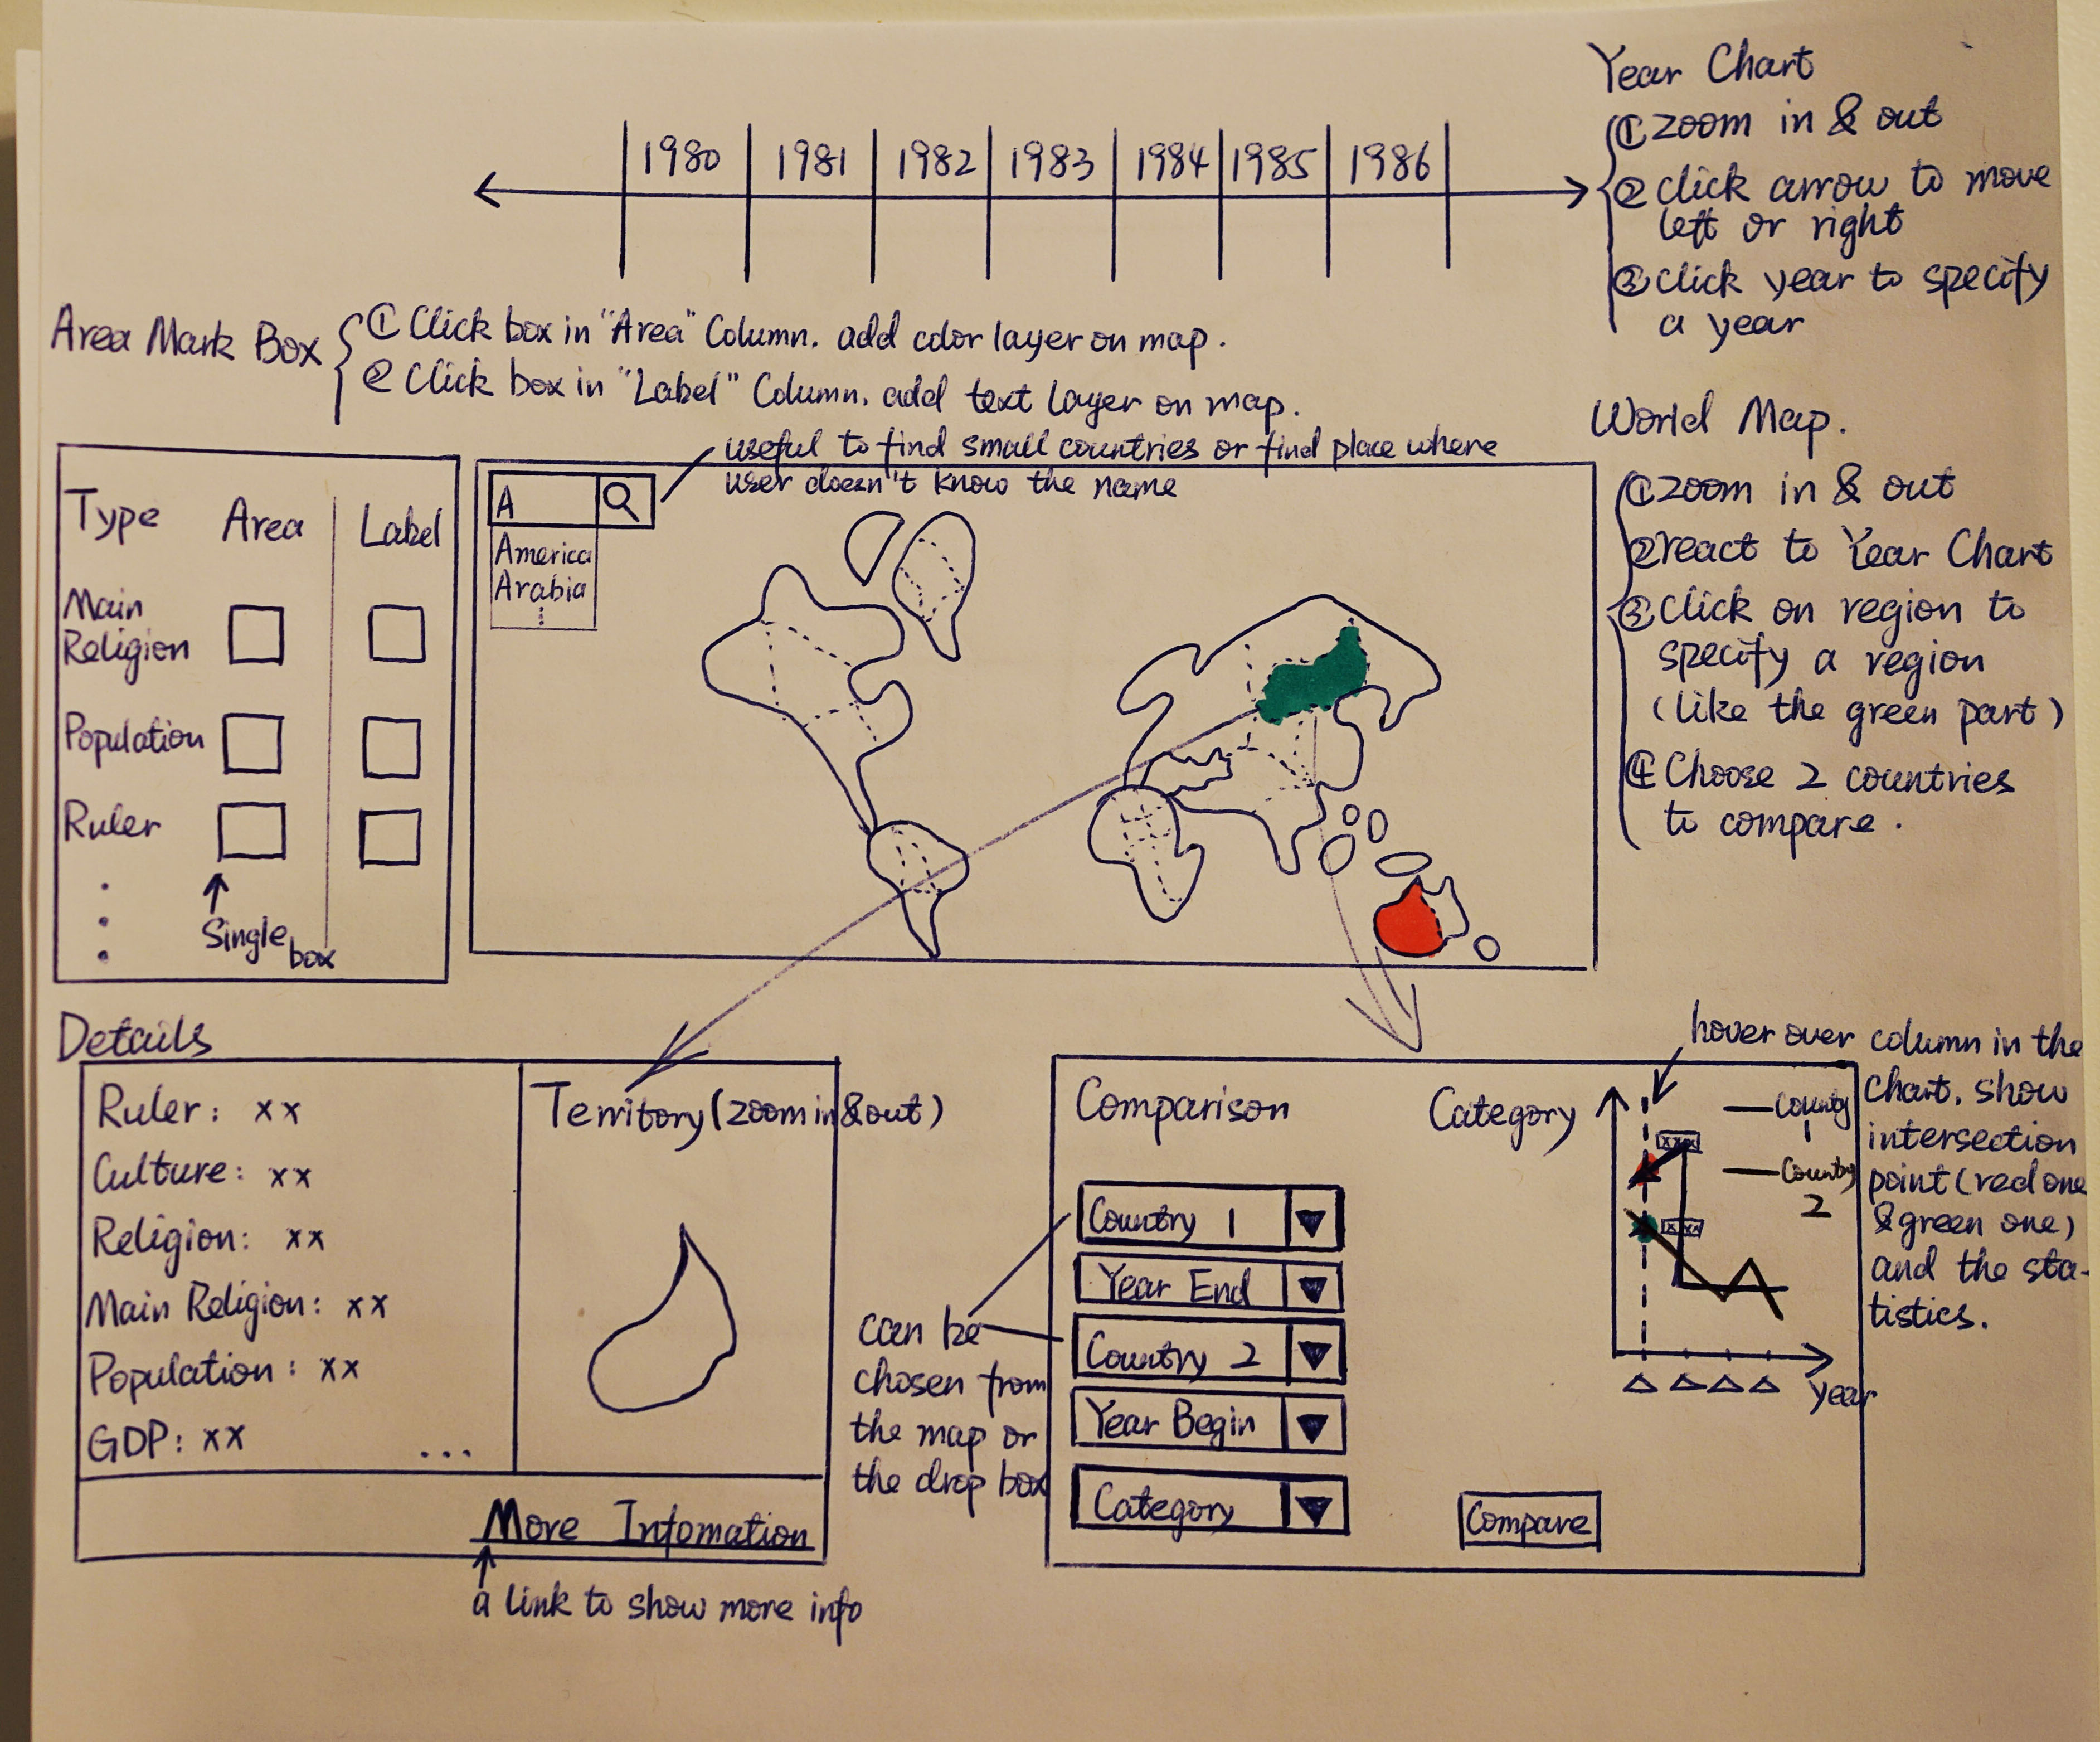
\includegraphics[width=\textwidth]{alternative3.JPG}
        \caption{Alternative 3}
        \label{fig:alt3}
    \end{center}
\end{figure}
\end{document}
